\documentclass[t, aspectratio=169]{beamer}
\usepackage{amsmath,amsfonts,amsthm,amstext,amssymb, xcolor, tikz, pgf, mathrsfs, polynom, pifont, tabto}

% ----------------------------------------------------------
% Theme Setup

% Use Metropolis Theme
\usetheme[numbering=fraction]{metropolis}
\setbeamertemplate{blocks}[rounded][shadow=false]
\makeatletter
\setlength{\metropolis@titleseparator@linewidth}{1pt}
\makeatother

% Define Colors
\definecolor{chargerblue}{HTML}{002764}
\definecolor{chargerred}{HTML}{e02034}
\definecolor{bggray}{HTML}{d0d3d4}

% Set Colors
\setbeamercolor{title}{fg=chargerblue}
\setbeamercolor{background canvas}{bg=white}
\setbeamercolor{title separator}{fg=chargerred}
\setbeamercolor{structure}{fg=chargerblue}
\setbeamercolor{frametitle}{fg=white, bg=chargerblue}
\setbeamercolor*{normal text}{fg=chargerblue}
\setbeamercolor*{block body}{bg=bggray}
\setbeamercolor*{block title}{bg=chargerblue, fg=white}
% ----------------------------------------------------------

% ----------------------------------------------------------
% Custom Definitions, Commands, Environments, etc.

% Sets of numbers
\def\R{\mathbb{R}} % The reals
\def\N{\mathbb{N}} % The naturals
\def\Z{\mathbb{Z}} % The integers
\def\Q{\mathbb{Q}} % The rationals

% Blank space
\newcommand{\blank}[1]{\underline{\hspace{#1}}} % Blank space

% Change font colors
\newcommand{\cyan}[1]{{\color{cyan}{#1}}} % Changes font to cyan
\newcommand{\red}[1]{{\color{red}{#1}}} % Changes font to red
\newcommand{\magenta}[1]{{\color{magenta}{#1}}} % Changes font to magenta
\newcommand{\orange}[1]{{\color{orange}{#1}}} % Changes font to orange
\newcommand{\yellow}[1]{{\color{yellow}{#1}}} % Changes font to yellow
\newcommand{\violet}[1]{{\color{violet}{#1}}} % Changes font to violet
\newcommand{\green}[1]{{\color{green}{#1}}} % Changes font to green
\newcommand{\blue}[1]{{\color{blue}{#1}}} % Changes font to blue
\newcommand{\white}[1]{{\color{white}{#1}}} % Changes font to white

% Fitted inclusion symbols
\newcommand{\fp}[1]{\left({#1}\right)} % Fitted parentheses around content
\newcommand{\fb}[1]{\left[{#1}\right]} % Fitted brackets
\newcommand{\lhoi}[1]{\left({#1}\right]} % Left half-open interval
\newcommand{\rhoi}[1]{\left[{#1}\right)} % Right half-open interval
\newcommand{\set}[1]{\left\{{#1}\right\}} % Fitted braces (useful for sets)
\newcommand{\av}[1]{\left|{#1}\right|} % Fitted absolute value bars

% Augmented Matrix Environment
\newenvironment{amatrix}[1]{%
	\left[\begin{array}{@{}*{#1}{c}|c@{}}
	}{%
	\end{array}\right]
}

% Miscellaneous
\def\then{\Rightarrow}
\def\to{\rightarrow}
\def\d{^{\circ}}
\newcommand{\?}{\stackrel{?}{=}}
\newcommand{\cmark}{\text{ \ding{51}}}
\newcommand{\xmark}{\text{ \ding{55}}}

% Coordinate Plane (Four-Quadrant)
\def\coordplane {
	\begin{tikzpicture}        \draw[step=0.25cm,black,very thin,opacity=0.25] (-2.5cm, -2.5cm) grid (2.5cm, 2.5cm);
		\draw[<->,thick,black] (-2.5cm, 0) -- (2.5cm, 0) node[anchor=north west,pos=0.94,font=\scriptsize]{$x$};
		\draw[<->,thick,black] (0,-2.5cm) -- (0, 2.5cm) node[anchor=south east,font=\scriptsize,pos=0.94]{$y$};
	\end{tikzpicture}
}

% Coordinate Plane (One-Quadrant)
\def\onequad {
	\begin{tikzpicture}
		\draw[step=0.25cm, black, very thin, opacity=0.25] (0,0) grid (7.5cm,5cm);
		\draw[->, thick, black] (0,0) -- (7.5cm, 0) node[anchor=north west,font=\scriptsize,pos=0.94]{$x$};
		\draw[->, black, thick] (0,0) -- (0,5cm) node[anchor=south east,font=\scriptsize,pos=0.94]{$y$};
	\end{tikzpicture}
}
% ----------------------------------------------------------

% ----------------------------------------------------------
% Presentation Information
\title[6-3]{The Central Limit Theorem}
\subtitle{Section 6-3}
\author{Jacob Ayers}
\institute{Lesson \#19}
\date{MAT 110}
% ----------------------------------------------------------

\begin{document}
	
	% Slide 1 (Title Slide)
	\begin{frame}
		\titlepage
	\end{frame}
	
	% Slide 2 (Objectives)
	\begin{frame}{Objectives}
		\begin{itemize}
			\item Use the Central Limit Theorem to solve problems involving sample means for large samples
		\end{itemize}
	\end{frame}

	\begin{frame}{The Central Limit Theorem}
		In the previous two lessons, we were interested in understanding how individual data values vary about the mean for a population. \pause
		
		Today, we shift our attention to studying how the means of samples of the same size vary about the population mean. \pause
		
		No two samples are likely to have exactly the same mean - there is variation in the sample means. \pause
		
		First, a couple terms:
		
		A \textit{sampling distribution of sample means} is a distribution using the means computed from all possible random samples of a specific size taken from a population. \pause
		
		\textit{Sampling error} is the difference between the sample measure and the corresponding population measure due to the fact that the sample is not a perfect representation of the population.
	\end{frame}

	\begin{frame}{The Central Limit Theorem}
		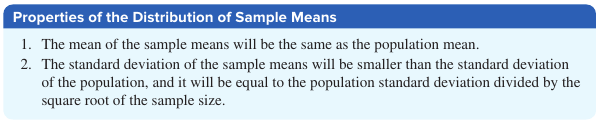
\includegraphics[width=\textwidth]{sample-mean-props} \pause
		
		Let's empirically confirm these properties through the use of an example.
	\end{frame}

	\begin{frame}{The Central Limit Theorem}
		Suppose I give an 8-point quiz to four students, who constitute the population. \pause
		
		Say their scores are $2$, $4$, $6$, and $8$. \pause
		
		Using a calculator, the mean is $5$ and the standard deviation is about $2.2361$. \pause
		
		Now, let's take all samples of size 2 (with replacement): \pause
		
		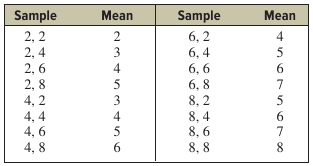
\includegraphics[width=3in]{clt-dist.png}
	\end{frame}

	\begin{frame}{The Central Limit Theorem}
		We can create a frequency distribution for the means, and use this to compute $\mu_{\overline{X}}$ and $\sigma_{\overline{X}}$. \pause
		
		Note on notation: $\mu_{\overline{X}}$ represents the \textit{mean of the sample means}, and $\sigma_{\overline{X}}$ represents the \textit{standard deviation of the sample means}.
		
		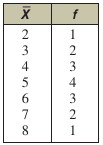
\includegraphics[width=1in]{clt-freq-dist.png}
	\end{frame}

	\begin{frame}{The Central Limit Theorem}
		Using a calculator, $\mu_{\overline{X}} = 5$ and $\sigma_{\overline{X}} \approx 1.5811$. \pause
		
		The properties stated that $\mu_{\overline{X}} = \mu$ (true) and $\sigma_{\overline{X}} = \dfrac{\sigma}{\sqrt{n}}$ (true, since $\dfrac{2.2361}{\sqrt{2}} \approx 1.5811$). \pause
		
		A final note before we get the Central Limit Theorem: the histogram appears to be approximately normal.
		
		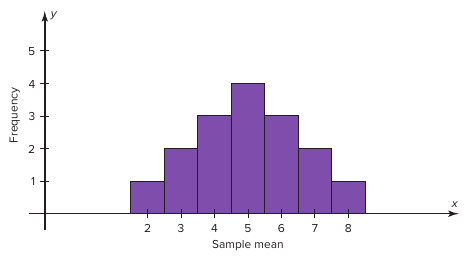
\includegraphics[width=3in]{clt-hist.png}
	\end{frame}

	\begin{frame}{The Central Limit Theorem}
		\begin{block}{The Central Limit Theorem}
			As the sample size $n$ increases without limit, the shape of the distribution of the sample means taken with replacement from a population with mean $\mu$ and standard deviation $\sigma$ will approach a normal distribution. This distribution will have a mean $\mu$ and standard deviation $\dfrac{\sigma}{\sqrt{n}}$.
		\end{block} \pause
	
		Takeaway: if the sample size is big enough, we can use the Central Limit Theorem to answer questions about sample means using the same strategies we used the normal distribution to answer questions about individual values. \pause
		
		Only difference: must use $z = \dfrac{\overline{X} - \mu}{\sigma / \sqrt{n}}$ to calculate $z$-score(s). \pause
		
		A calculator can be used once we have found the $z$-score(s).
	\end{frame}

	\begin{frame}{The Central Limit Theorem}
		A.C. Nielsen reported that children between the ages of 2 and 5 watch an average of 25 hours of television per week. Assume the variable is normally distributed and the standard deviation is 3 hours. If 20 children between the ages of 2 and 5 are randomly selected, find the probability that the mean of the number of hours they watch television will be greater than 26.7 hours. \pause
		
		Since the variable is approximately normally distributed, the distribution of sample means will be approximately normal with $\mu = 25$ and $\sigma = \dfrac{3}{\sqrt{20}} \approx 0.6708$.
	\end{frame}

	\begin{frame}{The Central Limit Theorem}
		First, draw a picture. \vspace{1in} \pause
		
		Now, compute the $z$-score: $z = \dfrac{26.7 - 25}{3 / \sqrt{20}} = \dfrac{1.7}{0.6708} \approx 2.53$. \pause
		
		So $P(\overline{X} > 26.7) = 1 - 0.9943 = 0.0057$.
	\end{frame}

	\begin{frame}{The Central Limit Theorem}
		The average lifetime of smoke detectors that a company manufactures is 60 months, with a standard deviation of 8 months. Find the probability that a random sample of 30 smoke detectors will have a mean lifetime between 58 and 63 months. \pause
		
		The distribution of sample means will be approximately normal, with $\mu = 60$ and $\sigma = \dfrac{8}{\sqrt{30}} \approx 1.4606$.
	\end{frame}

	\begin{frame}{The Central Limit Theorem}
		First, draw a picture. \vspace{1in} \pause
		
		Now, compute the $z$-scores: \\
		Lower: $z = \dfrac{58 - 60}{8 / \sqrt{30}} = \dfrac{-2}{1.4606} \approx -1.37$. \pause \\
		Upper: $z = \dfrac{63 - 60}{8 / \sqrt{30}} = \dfrac{3}{1.4606} \approx 2.05$ \pause
		
		So $P(58 < \overline{X} < 63) = 0.9798 - 0.0853 = 0.8945$.
	\end{frame}

	\begin{frame}{The Central Limit Theorem}
		The average number of moves a person makes in his or her lifetime is 12. If the standard deviation is 3.2, find the probability that the mean of a sample of 36 people is less than 11. \pause
		
		The distribution of sample means will be approximately normal, with $\mu = 12$ and $\sigma = \dfrac{3.2}{\sqrt{36}} \approx 0.5333$.
	\end{frame}

	\begin{frame}{The Central Limit Theorem}
		First, draw a picture. \pause \vspace{1in}
		
		Now, compute the $z$-score: $z = \dfrac{11 - 12}{3.2 / \sqrt{36}} = \dfrac{-1}{0.5333} \approx -1.88$. \pause
		
		So $P(\overline{X} < 11) = 0.0301$
	\end{frame}

	\begin{frame}{Next Steps}
		\begin{itemize}
			\item Complete Assignment \#9
			\item Begin Module \#11 \begin{itemize}
				\item Read 7-1
				\item Watch Video Lesson \#20
			\end{itemize}
		\end{itemize}
		
		\vfill
		
		Thanks for watching!
	\end{frame}
	
\end{document}